\documentclass[a4paper,11pt]{article}


% define the title
\author{Xue, Yuan}
\title{Assignment 5 Packet}


\usepackage{verbatim}
\usepackage{amsmath}
\usepackage{amssymb}
%\usepackage{tikz}
%\usetikzlibrary{graphs}
\usepackage{graphicx}
\usepackage{caption}
\usepackage{subcaption}

%\pagestyle{headings}
%\thispagestyle{headings}

\begin{document}
\maketitle

\subsection*{Question A.1}

From Figure \ref{fig:A1} we see that the distribution of birth weights is not smooth. It more clusters in some bins.

\begin{figure}[h]
\centering
\begin{subfigure}{.33\textwidth}
  \centering
  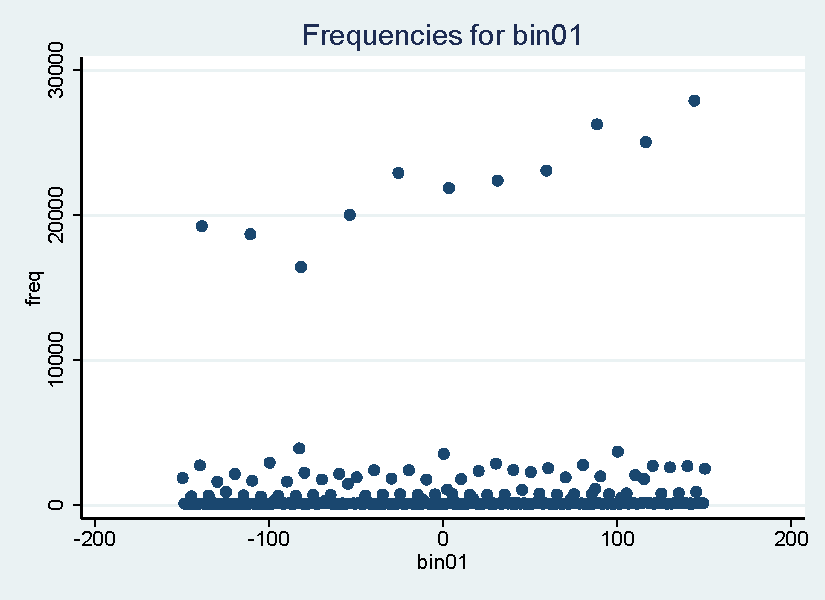
\includegraphics[width=\linewidth]{graph_bin01.pdf}
  \caption{Bin Length: 01 gram}
  \label{fig:sub1}
\end{subfigure}%
\begin{subfigure}{.33\textwidth}
  \centering
  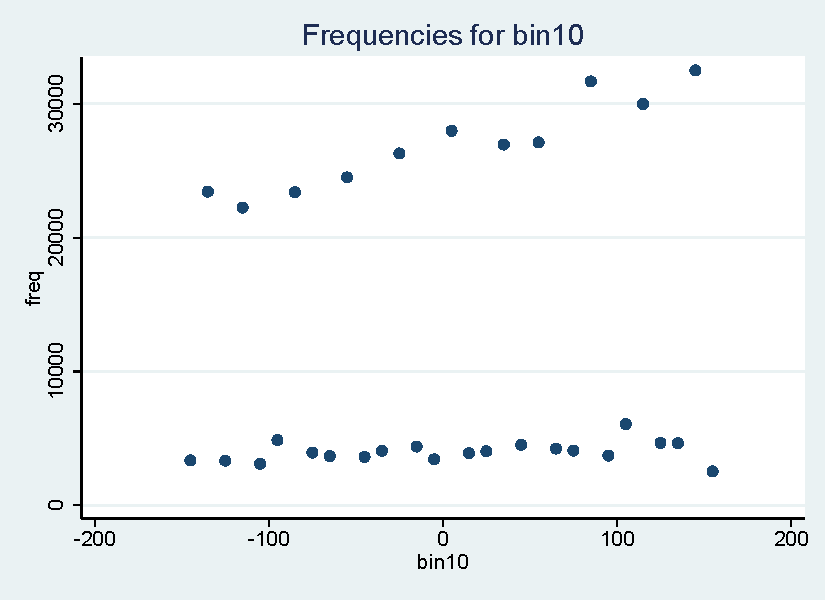
\includegraphics[width=\linewidth]{graph_bin10.pdf}
  \caption{Bin Length: 10 gram}
  \label{fig:sub2}
\end{subfigure}
\begin{subfigure}{.33\textwidth}
  \centering
  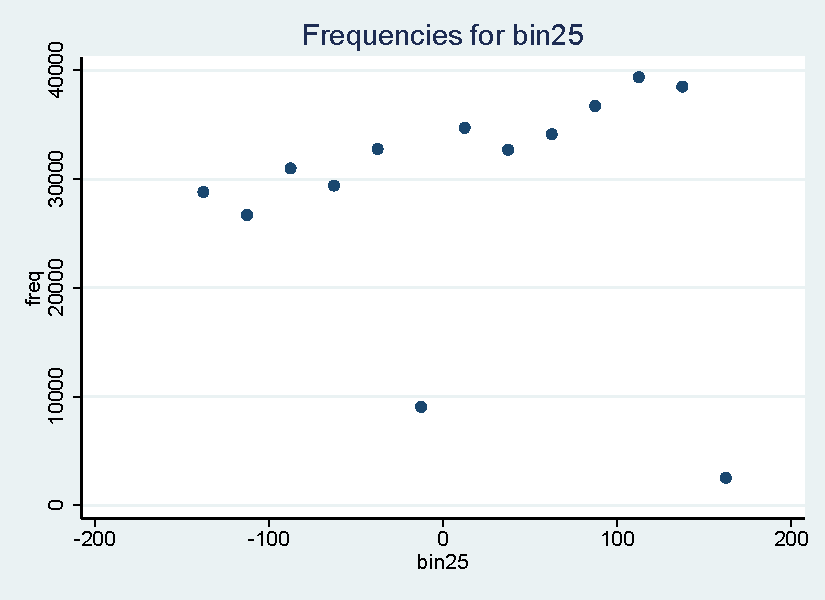
\includegraphics[width=1\linewidth]{graph_bin25.pdf}
  \caption{Bin Length: 25 gram}
  \label{fig:sub3}
\end{subfigure}
\caption{Frequencies of bins with different lengths}
\label{fig:A1}
\end{figure}

\subsection*{Question A.2}

From table \ref{A2.bin01}, table \ref{A2.bin10}
and table \ref{A2.bin25} we basically observe no significant discontinuity of the frequencies of running variable pre and post the cutoff. However, we can see a jump on the intercept when the bandwidth is 150 on 90\% significance level.

%%%%%%%%%%%%%%%%%%%%%%bin01%%%%%%%%%%%%%%%%%%%
\begin{table}[htbp]\centering
\def\sym#1{\ifmmode^{#1}\else\(^{#1}\)\fi}
\caption{Test continuity via frequency, bin01}
\label{A2.bin01}
\begin{tabular}{l*{3}{c}}
\hline\hline
            &\multicolumn{1}{c}{bandwidth:150}&\multicolumn{1}{c}{bandwidth:100}&\multicolumn{1}{c}{bandwidth:50}\\
\hline
cut         &      -447.2         &      -740.2         &     -1611.6         \\
            &     (-0.46)         &     (-0.64)         &     (-1.04)         \\
[1em]
bin01       &       1.124         &      -4.347         &      -38.87         \\
            &      (0.14)         &     (-0.31)         &     (-1.03)         \\
[1em]
inter       &      -3.018         &       1.099         &       33.74         \\
            &     (-0.27)         &      (0.06)         &      (0.63)         \\
[1em]
\_cons      &      1356.6\sym{**} &      1600.0\sym{*}  &      2319.9\sym{**} \\
            &      (1.97)         &      (1.97)         &      (2.12)         \\
\hline
\(N\)       &         300         &         200         &         100         \\
\hline\hline
\multicolumn{4}{l}{\footnotesize \textit{t} statistics in parentheses}\\
\multicolumn{4}{l}{\footnotesize \sym{*} \(p<0.10\), \sym{**} \(p<0.05\), \sym{***} \(p<0.01\)}\\
\end{tabular}
\end{table}


%%%%%%%%%%%%%%%%%%%%%bin10%%%%%%%%%%%%%%%%%%%%%%%%%%%

\begin{table}[htbp]\centering
\def\sym#1{\ifmmode^{#1}\else\(^{#1}\)\fi}
\caption{Test continuity via frequency, bin10}
\label{A2.bin10}
\begin{tabular}{l*{3}{c}}
\hline\hline
            &\multicolumn{1}{c}{bandwidth:150}&\multicolumn{1}{c}{bandwidth:100}&\multicolumn{1}{c}{bandwidth:50}\\
\hline
cut         &     -4270.2         &     -7335.8         &    -11093.7         \\
            &     (-0.49)         &     (-0.68)         &     (-0.67)         \\
[1em]
bin10       &       13.07         &      -41.96         &      -238.6         \\
            &      (0.19)         &     (-0.32)         &     (-0.58)         \\
[1em]
inter       &      -31.16         &       9.290         &       238.2         \\
            &     (-0.31)         &      (0.05)         &      (0.41)         \\
[1em]
\_cons      &     13429.1\sym{**} &     15924.7\sym{*}  &     19447.9         \\
            &      (2.20)         &      (2.08)         &      (1.66)         \\
\hline
\(N\)       &          30         &          20         &          10         \\
\hline\hline
\multicolumn{4}{l}{\footnotesize \textit{t} statistics in parentheses}\\
\multicolumn{4}{l}{\footnotesize \sym{*} \(p<0.10\), \sym{**} \(p<0.05\), \sym{***} \(p<0.01\)}\\
\end{tabular}
\end{table}


%%%%%%%%%%%%%%%%%%%%bin25%%%%%%%%%%%%%%%%%%%%%%%%

\begin{table}[htbp]\centering
\def\sym#1{\ifmmode^{#1}\else\(^{#1}\)\fi}
\caption{Test continuity via frequency, bin25}
\label{A2.bin25}
\begin{tabular}{l*{3}{c}}
\hline\hline
            &\multicolumn{1}{c}{bandwidth:150}&\multicolumn{1}{c}{bandwidth:100}&\multicolumn{1}{c}{bandwidth:50}\\
\hline
cut         &    -13216.7\sym{*}  &    -20013.0         &    -38534.5         \\
            &     (-1.88)         &     (-2.06)         &         (.)         \\
[1em]
bin25       &       47.48         &       29.84         &      -80.92         \\
            &      (0.82)         &      (0.25)         &         (.)         \\
[1em]
inter       &      -141.4         &      -279.7         &      -867.7         \\
            &     (-1.73)         &     (-1.65)         &         (.)         \\
[1em]
\_cons      &     32462.2\sym{***}&     33075.0\sym{***}&     35729.5         \\
            &      (6.53)         &      (4.82)         &         (.)         \\
\hline
\(N\)       &          12         &           8         &           4         \\
\hline\hline
\multicolumn{4}{l}{\footnotesize \textit{t} statistics in parentheses}\\
\multicolumn{4}{l}{\footnotesize \sym{*} \(p<0.10\), \sym{**} \(p<0.05\), \sym{***} \(p<0.01\)}\\
\end{tabular}
\end{table}

\subsection*{Question A.3}

From table \ref{A3.bw90}, table \ref{A3.bw60} and table \ref{A3.bw30}, we can see that with larger bandwidth (90 gram), both the race of mom and the education level of mom are discontinuous on the slopes. As the bandwidth goes smaller, the race of mom losts discontinuity on the slopes, but the education of mom keeps the discontinuity. Therefore the results are sensitive to bandwidth.

We can also observe that rectangular kernel is usually more able to capture the discontinuity.

We can guess from data that since mom's education level slope becomes flat after cutoff, then before the cutoff, the more educated mom tends to push to keep their babies in the program. The same logic may apply to non-white mom. This confounder may harm the validity of our regression discontinuity method.


%%%%%%%%%%%%%%%%%%%%%%%%%%bw 90%%%%%%%%%%%%%%%

\begin{table}[htbp]\centering
\def\sym#1{\ifmmode^{#1}\else\(^{#1}\)\fi}
\caption{Test continuity via characteristics, bandwidth: 90}
\label{A3.bw90}
\begin{tabular}{l*{4}{c}}
\hline\hline
            &\multicolumn{1}{c}{mom\_white\_TK}&\multicolumn{1}{c}{mom\_white\_RK}&\multicolumn{1}{c}{mom\_high\_TK}&\multicolumn{1}{c}{mom\_high\_RK}\\
\hline
bwtnorm     &   -0.000110         &  -0.0000360         &   0.0000512         &   0.0000323         \\
            &     (-1.33)         &     (-0.57)         &      (0.68)         &      (0.56)         \\
[1em]
cut         &     0.00482         &     0.00120         &     0.00209         &     0.00182         \\
            &      (1.01)         &      (0.28)         &      (0.48)         &      (0.47)         \\
[1em]
inter       &    0.000188\sym{*}  &    0.000154\sym{**} &   -0.000177\sym{*}  &   -0.000119\sym{*}  \\
            &      (1.82)         &      (2.05)         &     (-1.87)         &     (-1.73)         \\
[1em]
\_cons      &       0.654\sym{***}&       0.657\sym{***}&       0.253\sym{***}&       0.252\sym{***}\\
            &    (161.81)         &    (185.54)         &     (68.26)         &     (77.81)         \\
\hline
\(N\)       &      230248         &      233887         &      230248         &      233887         \\
\hline\hline
\multicolumn{5}{l}{\footnotesize \textit{t} statistics in parentheses}\\
\multicolumn{5}{l}{\footnotesize \sym{*} \(p<0.10\), \sym{**} \(p<0.05\), \sym{***} \(p<0.01\)}\\
\end{tabular}
\end{table}


%%%%%%%%%%%%%%%%%%%%%%%%%%bw 60%%%%%%%%%%%%%%%

\begin{table}[htbp]\centering
\def\sym#1{\ifmmode^{#1}\else\(^{#1}\)\fi}
\caption{Test continuity via characteristics, bandwidth: 60}
\label{A3.bw60}
\begin{tabular}{l*{4}{c}}
\hline\hline
            &\multicolumn{1}{c}{mom\_white\_TK}&\multicolumn{1}{c}{mom\_white\_RK}&\multicolumn{1}{c}{mom\_high\_TK}&\multicolumn{1}{c}{mom\_high\_RK}\\
\hline
bwtnorm     &   -0.000220         &   -0.000215\sym{*}  &    0.000202         &   0.0000210         \\
            &     (-1.35)         &     (-1.82)         &      (1.35)         &      (0.19)         \\
[1em]
cut         &     0.00843         &     0.00673         &    -0.00174         &     0.00385         \\
            &      (1.33)         &      (1.24)         &     (-0.30)         &      (0.78)         \\
[1em]
inter       &    0.000240         &    0.000345\sym{**} &   -0.000314\sym{*}  &   -0.000188         \\
            &      (1.21)         &      (2.52)         &     (-1.72)         &     (-1.50)         \\
[1em]
\_cons      &       0.651\sym{***}&       0.651\sym{***}&       0.256\sym{***}&       0.252\sym{***}\\
            &    (115.85)         &    (136.78)         &     (49.64)         &     (57.75)         \\
\hline
\(N\)       &      158693         &      163422         &      158693         &      163422         \\
\hline\hline
\multicolumn{5}{l}{\footnotesize \textit{t} statistics in parentheses}\\
\multicolumn{5}{l}{\footnotesize \sym{*} \(p<0.10\), \sym{**} \(p<0.05\), \sym{***} \(p<0.01\)}\\
\end{tabular}
\end{table}

%%%%%%%%%%%%%%%%%%%%%%%%%%bw 30%%%%%%%%%%%%%%%
\begin{table}[htbp]\centering
\def\sym#1{\ifmmode^{#1}\else\(^{#1}\)\fi}
\caption{Test continuity via characteristics, bandwidth: 30}
\label{A3.bw30}
\begin{tabular}{l*{4}{c}}
\hline\hline
            &\multicolumn{1}{c}{mom\_white\_TK}&\multicolumn{1}{c}{mom\_white\_RK}&\multicolumn{1}{c}{mom\_high\_TK}&\multicolumn{1}{c}{mom\_high\_RK}\\
\hline
bwtnorm     &   -0.000179         &   -0.000409         &    0.000546         &    0.000682\sym{*}  \\
            &     (-0.39)         &     (-0.99)         &      (1.29)         &      (1.81)         \\
[1em]
cut         &     0.00712         &      0.0165         &    -0.00734         &     -0.0115         \\
            &      (0.64)         &      (1.59)         &     (-0.72)         &     (-1.21)         \\
[1em]
inter       &    0.000397         &   -0.000689         &    -0.00107\sym{*}  &   -0.000776\sym{*}  \\
            &      (0.63)         &     (-1.40)         &     (-1.86)         &     (-1.73)         \\
[1em]
\_cons      &       0.652\sym{***}&       0.647\sym{***}&       0.264\sym{***}&       0.266\sym{***}\\
            &     (61.88)         &     (65.29)         &     (27.10)         &     (29.33)         \\
\hline
\(N\)       &       68207         &       72941         &       68207         &       72941         \\
\hline\hline
\multicolumn{5}{l}{\footnotesize \textit{t} statistics in parentheses}\\
\multicolumn{5}{l}{\footnotesize \sym{*} \(p<0.10\), \sym{**} \(p<0.05\), \sym{***} \(p<0.01\)}\\
\end{tabular}
\end{table}

\subsection*{Question A.4}

From table \ref{A4.oz51}, table \ref{A4.oz52}, table \ref{A4.oz53} and table \ref{A4.oz54}, we can observe that infants at the ounce heaps are more possible to have a white mom. However, there are basically no significant jumps on mom's education level for those ounce heap infants.

From table \ref{A4.1500}, we can observe that the infants heaping at 1500 gram are less likely to have a white mom, but are more likely to have a mom at least having a high school level education.

%%%%%%%%%%%%%%%%%%%%%%%%% 51 %%%%%%%%%%%%%%%%%%%%%%

\begin{table}[htbp]\centering
\def\sym#1{\ifmmode^{#1}\else\(^{#1}\)\fi}
\caption{Test jump on oz 51, bandwidth: 25}
\label{A4.oz51}
\begin{tabular}{l*{2}{c}}
\hline\hline
            &\multicolumn{1}{c}{mom\_white}&\multicolumn{1}{c}{mom\_high}\\
\hline
bweight     &   -0.000169         &  -0.0000465         \\
            &     (-0.70)         &     (-0.21)         \\
[1em]
inter51     &   0.0000185\sym{***}&-0.000000925         \\
            &      (5.58)         &     (-0.31)         \\
[1em]
\_cons      &       0.890\sym{**} &       0.319         \\
            &      (2.55)         &      (1.00)         \\
\hline
\(N\)       &       39519         &       39519         \\
\hline\hline
\multicolumn{3}{l}{\footnotesize \textit{t} statistics in parentheses}\\
\multicolumn{3}{l}{\footnotesize \sym{*} \(p<0.10\), \sym{**} \(p<0.05\), \sym{***} \(p<0.01\)}\\
\end{tabular}
\end{table}


%%%%%%%%%%%%%%%%%%%%%%%%% 52 %%%%%%%%%%%%%%%%%%%%%%

\begin{table}[htbp]\centering
\def\sym#1{\ifmmode^{#1}\else\(^{#1}\)\fi}
\caption{Test jump on oz 52, bandwidth: 25}
\label{A4.oz52}
\begin{tabular}{l*{2}{c}}
\hline\hline
            &\multicolumn{1}{c}{mom\_white}&\multicolumn{1}{c}{mom\_high}\\
\hline
bweight     &    0.000170         &    0.000228         \\
            &      (0.71)         &      (1.04)         \\
[1em]
inter52     &   0.0000135\sym{***}& -0.00000460         \\
            &      (4.24)         &     (-1.59)         \\
[1em]
\_cons      &       0.393         &     -0.0810         \\
            &      (1.12)         &     (-0.25)         \\
\hline
\(N\)       &       41928         &       41928         \\
\hline\hline
\multicolumn{3}{l}{\footnotesize \textit{t} statistics in parentheses}\\
\multicolumn{3}{l}{\footnotesize \sym{*} \(p<0.10\), \sym{**} \(p<0.05\), \sym{***} \(p<0.01\)}\\
\end{tabular}
\end{table}


%%%%%%%%%%%%%%%%%%%%%%%%% 53 %%%%%%%%%%%%%%%%%%%%%%

\begin{table}[htbp]\centering
\def\sym#1{\ifmmode^{#1}\else\(^{#1}\)\fi}
\caption{Test jump on oz 53, bandwidth: 25}
\label{A4.oz53}
\begin{tabular}{l*{2}{c}}
\hline\hline
            &\multicolumn{1}{c}{mom\_white}&\multicolumn{1}{c}{mom\_high}\\
\hline
bweight     &    0.000516\sym{**} &   -0.000353\sym{*}  \\
            &      (2.26)         &     (-1.68)         \\
[1em]
inter53     &   0.0000186\sym{***}&  0.00000120         \\
            &      (5.90)         &      (0.41)         \\
[1em]
\_cons      &      -0.131         &       0.782\sym{**} \\
            &     (-0.38)         &      (2.49)         \\
\hline
\(N\)       &       40358         &       40358         \\
\hline\hline
\multicolumn{3}{l}{\footnotesize \textit{t} statistics in parentheses}\\
\multicolumn{3}{l}{\footnotesize \sym{*} \(p<0.10\), \sym{**} \(p<0.05\), \sym{***} \(p<0.01\)}\\
\end{tabular}
\end{table}


%%%%%%%%%%%%%%%%%%%%%%%%% 54 %%%%%%%%%%%%%%%%%%%%%%

\begin{table}[htbp]\centering
\def\sym#1{\ifmmode^{#1}\else\(^{#1}\)\fi}
\caption{Test jump on oz 54, bandwidth: 25}
\label{A4.oz54}
\begin{tabular}{l*{2}{c}}
\hline\hline
            &\multicolumn{1}{c}{mom\_white}&\multicolumn{1}{c}{mom\_high}\\
\hline
bweight     &    0.000215         &    0.000145         \\
            &      (0.93)         &      (0.68)         \\
[1em]
inter54     &   0.0000147\sym{***}& -0.00000186         \\
            &      (4.94)         &     (-0.68)         \\
[1em]
\_cons      &       0.317         &      0.0314         \\
            &      (0.89)         &      (0.10)         \\
\hline
\(N\)       &       43655         &       43655         \\
\hline\hline
\multicolumn{3}{l}{\footnotesize \textit{t} statistics in parentheses}\\
\multicolumn{3}{l}{\footnotesize \sym{*} \(p<0.10\), \sym{**} \(p<0.05\), \sym{***} \(p<0.01\)}\\
\end{tabular}
\end{table}

%%%%%%%%%%%%%%%%%%%% 1500 %%%%%%%%%%%%%%%%%%%%%%%%

\begin{table}[htbp]\centering
\def\sym#1{\ifmmode^{#1}\else\(^{#1}\)\fi}
\caption{Test jump on 1500, bandwidth: 25}
\label{A4.1500}
\begin{tabular}{l*{2}{c}}
\hline\hline
            &\multicolumn{1}{c}{mom\_white}&\multicolumn{1}{c}{mom\_high}\\
\hline
bweight     &    0.000292         &   -0.000132         \\
            &      (1.32)         &     (-0.66)         \\
[1em]
inter2      &  -0.0000137\sym{**} &   0.0000116\sym{**} \\
            &     (-2.34)         &      (2.18)         \\
[1em]
\_cons      &       0.206         &       0.450         \\
            &      (0.62)         &      (1.49)         \\
\hline
\(N\)       &       22613         &       22613         \\
\hline\hline
\multicolumn{3}{l}{\footnotesize \textit{t} statistics in parentheses}\\
\multicolumn{3}{l}{\footnotesize \sym{*} \(p<0.10\), \sym{**} \(p<0.05\), \sym{***} \(p<0.01\)}\\
\end{tabular}
\end{table}

\subsection*{Question B.1}

From table \ref{B1.bw90}, table \ref{B1.bw60}, table \ref{B1.bw30}, we can observe obvious effect of cutoff of birth weight on mortality. We can observe even stronger effects on both intercept and slope as brandwidth becomes smaller and use the triangular kernel method.

%%%%%%%%%%%%%%%%%%%%%%%%% bw 90 %%%%%%%%%%%%

\begin{table}[htbp]\centering
\def\sym#1{\ifmmode^{#1}\else\(^{#1}\)\fi}
\caption{Birth weight class on mortality, bandwidth: 90}
\label{B1.bw90}
\begin{tabular}{l*{2}{c}}
\hline\hline
            &\multicolumn{1}{c}{Triangular}&\multicolumn{1}{c}{Rectangular}\\
\hline
bwtnorm     &   -0.000166\sym{***}&   -0.000128\sym{***}\\
            &     (-4.19)         &     (-4.06)         \\
[1em]
cut         &      0.0114\sym{***}&     0.00737\sym{***}\\
            &      (4.86)         &      (3.53)         \\
[1em]
inter       &  -0.0000858\sym{*}  &  -0.0000175         \\
            &     (-1.70)         &     (-0.47)         \\
[1em]
\_cons      &      0.0525\sym{***}&      0.0539\sym{***}\\
            &     (27.28)         &     (31.02)         \\
\hline
\(N\)       &      230248         &      233887         \\
\hline\hline
\multicolumn{3}{l}{\footnotesize \textit{t} statistics in parentheses}\\
\multicolumn{3}{l}{\footnotesize \sym{*} \(p<0.10\), \sym{**} \(p<0.05\), \sym{***} \(p<0.01\)}\\
\end{tabular}
\end{table}


%%%%%%%%%%%%%%%%%%%%%%%%% bw 60 %%%%%%%%%%%%

\begin{table}[htbp]\centering
\def\sym#1{\ifmmode^{#1}\else\(^{#1}\)\fi}
\caption{Birth weight class on mortality, bandwidth: 60}
\label{B1.bw60}
\begin{tabular}{l*{2}{c}}
\hline\hline
            &\multicolumn{1}{c}{Triangular}&\multicolumn{1}{c}{Rectangular}\\
\hline
bwtnorm     &   -0.000279\sym{***}&   -0.000184\sym{***}\\
            &     (-3.69)         &     (-3.16)         \\
[1em]
cut         &      0.0161\sym{***}&      0.0110\sym{***}\\
            &      (5.34)         &      (4.13)         \\
[1em]
inter       &   -0.000128         &  -0.0000431         \\
            &     (-1.35)         &     (-0.64)         \\
[1em]
\_cons      &      0.0497\sym{***}&      0.0522\sym{***}\\
            &     (19.08)         &     (22.64)         \\
\hline
\(N\)       &      158693         &      163422         \\
\hline\hline
\multicolumn{3}{l}{\footnotesize \textit{t} statistics in parentheses}\\
\multicolumn{3}{l}{\footnotesize \sym{*} \(p<0.10\), \sym{**} \(p<0.05\), \sym{***} \(p<0.01\)}\\
\end{tabular}
\end{table}


%%%%%%%%%%%%%%%%%%%%%%%%% bw 30 %%%%%%%%%%%%

\begin{table}[htbp]\centering
\def\sym#1{\ifmmode^{#1}\else\(^{#1}\)\fi}
\caption{Birth weight class on mortality, bandwidth: 30}
\label{B1.bw30}
\begin{tabular}{l*{2}{c}}
\hline\hline
            &\multicolumn{1}{c}{Triangular}&\multicolumn{1}{c}{Rectangular}\\
\hline
bwtnorm     &   -0.000554\sym{***}&   -0.000464\sym{**} \\
            &     (-2.67)         &     (-2.44)         \\
[1em]
cut         &      0.0263\sym{***}&      0.0214\sym{***}\\
            &      (5.18)         &      (4.43)         \\
[1em]
inter       &    -0.00112\sym{***}&   -0.000394\sym{*}  \\
            &     (-3.76)         &     (-1.73)         \\
[1em]
\_cons      &      0.0445\sym{***}&      0.0461\sym{***}\\
            &      (9.43)         &     (10.18)         \\
\hline
\(N\)       &       68207         &       72941         \\
\hline\hline
\multicolumn{3}{l}{\footnotesize \textit{t} statistics in parentheses}\\
\multicolumn{3}{l}{\footnotesize \sym{*} \(p<0.10\), \sym{**} \(p<0.05\), \sym{***} \(p<0.01\)}\\
\end{tabular}
\end{table}

\subsection*{Question B.2}

From table \ref{B2.bw90}, table \ref{B2.bw60}, table \ref{B2.bw30}, we can observe that the cutoff effect loses its significance on slope differences. But we still can get a lower one year death rate if the infants are assigned to the less than 1500 gram group.

%%%%%%%%%%%%%%%%%%% 90%%%%%%%%%%%%%%%%%%%%%%%%%

\begin{table}[htbp]\centering
\def\sym#1{\ifmmode^{#1}\else\(^{#1}\)\fi}
\caption{Birth weight class on mortality, bandwidth: 90 , 1500 dropped}
\label{B2.bw90}
\begin{tabular}{l*{2}{c}}
\hline\hline
            &\multicolumn{1}{c}{Triangular}&\multicolumn{1}{c}{Rectangular}\\
\hline
bwtnorm     &   -0.000166\sym{***}&   -0.000128\sym{***}\\
            &     (-4.19)         &     (-4.06)         \\
[1em]
cut         &     0.00650\sym{***}&     0.00376\sym{*}  \\
            &      (2.77)         &      (1.79)         \\
[1em]
inter       &   0.0000226         &   0.0000365         \\
            &      (0.45)         &      (0.97)         \\
[1em]
\_cons      &      0.0525\sym{***}&      0.0539\sym{***}\\
            &     (27.28)         &     (31.02)         \\
\hline
\(N\)       &      226704         &      230343         \\
\hline\hline
\multicolumn{3}{l}{\footnotesize \textit{t} statistics in parentheses}\\
\multicolumn{3}{l}{\footnotesize \sym{*} \(p<0.10\), \sym{**} \(p<0.05\), \sym{***} \(p<0.01\)}\\
\end{tabular}
\end{table}


%%%%%%%%%%%%%%%%%%% 60%%%%%%%%%%%%%%%%%%%%%%%%%

\begin{table}[htbp]\centering
\def\sym#1{\ifmmode^{#1}\else\(^{#1}\)\fi}
\caption{Birth weight class on mortality, bandwidth: 60 , 1500 dropped}
\label{B2.bw60}
\begin{tabular}{l*{2}{c}}
\hline\hline
            &\multicolumn{1}{c}{Triangular}&\multicolumn{1}{c}{Rectangular}\\
\hline
bwtnorm     &   -0.000279\sym{***}&   -0.000184\sym{***}\\
            &     (-3.69)         &     (-3.16)         \\
[1em]
cut         &      0.0101\sym{***}&     0.00648\sym{**} \\
            &      (3.34)         &      (2.42)         \\
[1em]
inter       &   0.0000771         &   0.0000544         \\
            &      (0.81)         &      (0.80)         \\
[1em]
\_cons      &      0.0497\sym{***}&      0.0522\sym{***}\\
            &     (19.08)         &     (22.64)         \\
\hline
\(N\)       &      155149         &      159878         \\
\hline\hline
\multicolumn{3}{l}{\footnotesize \textit{t} statistics in parentheses}\\
\multicolumn{3}{l}{\footnotesize \sym{*} \(p<0.10\), \sym{**} \(p<0.05\), \sym{***} \(p<0.01\)}\\
\end{tabular}
\end{table}


%%%%%%%%%%%%%%%%%%% 30%%%%%%%%%%%%%%%%%%%%%%%%%

\begin{table}[htbp]\centering
\def\sym#1{\ifmmode^{#1}\else\(^{#1}\)\fi}
\caption{Birth weight class on mortality, bandwidth: 30 , 1500 dropped}
\label{B2.bw30}
\begin{tabular}{l*{2}{c}}
\hline\hline
            &\multicolumn{1}{c}{Triangular}&\multicolumn{1}{c}{Rectangular}\\
\hline
bwtnorm     &   -0.000554\sym{***}&   -0.000464\sym{**} \\
            &     (-2.67)         &     (-2.44)         \\
[1em]
cut         &      0.0175\sym{***}&      0.0151\sym{***}\\
            &      (3.45)         &      (3.12)         \\
[1em]
inter       &   -0.000153         &  -0.0000515         \\
            &     (-0.53)         &     (-0.22)         \\
[1em]
\_cons      &      0.0445\sym{***}&      0.0461\sym{***}\\
            &      (9.43)         &     (10.18)         \\
\hline
\(N\)       &       64663         &       69397         \\
\hline\hline
\multicolumn{3}{l}{\footnotesize \textit{t} statistics in parentheses}\\
\multicolumn{3}{l}{\footnotesize \sym{*} \(p<0.10\), \sym{**} \(p<0.05\), \sym{***} \(p<0.01\)}\\
\end{tabular}
\end{table}

\subsection*{Question B.3}

From table \ref{B3.bw90}, table \ref{B3.bw60}, table \ref{B3.bw30}, we notice that by dropping 1500 and ounce heaps, we almost lost all cutoff effects. The exception is that, with 90 bandwidth, we still could see a higher slope for the infants who is close but above the 1500 gram cutoff, which means without further care, the mortality grows faster as baby's weight gets less.

%%%%%%%%%%%%%%%%%% 90 %%%%%%%%%%%%%%%%%%%%%%%%%%

\begin{table}[htbp]\centering
\def\sym#1{\ifmmode^{#1}\else\(^{#1}\)\fi}
\caption{Birth weight class on mortality, bandwidth: 90 , 1500 and ounce heaps dropped}
\label{B3.bw90}
\begin{tabular}{l*{2}{c}}
\hline\hline
            &\multicolumn{1}{c}{Triangular}&\multicolumn{1}{c}{Rectangular}\\
\hline
bwtnorm     &   -0.000170\sym{***}&   -0.000169\sym{***}\\
            &     (-3.73)         &     (-4.49)         \\
[1em]
cut         &     0.00118         &    0.000866         \\
            &      (0.33)         &      (0.27)         \\
[1em]
inter       &    0.000168\sym{***}&    0.000174\sym{***}\\
            &      (2.60)         &      (3.61)         \\
[1em]
\_cons      &      0.0497\sym{***}&      0.0497\sym{***}\\
            &     (19.30)         &     (20.53)         \\
\hline
\(N\)       &      139461         &      143100         \\
\hline\hline
\multicolumn{3}{l}{\footnotesize \textit{t} statistics in parentheses}\\
\multicolumn{3}{l}{\footnotesize \sym{*} \(p<0.10\), \sym{**} \(p<0.05\), \sym{***} \(p<0.01\)}\\
\end{tabular}
\end{table}


%%%%%%%%%%%%%%%%%% 60 %%%%%%%%%%%%%%%%%%%%%%%%%%

\begin{table}[htbp]\centering
\def\sym#1{\ifmmode^{#1}\else\(^{#1}\)\fi}
\caption{Birth weight class on mortality, bandwidth: 60 , 1500 and ounce heaps dropped}
\label{B3.bw60}
\begin{tabular}{l*{2}{c}}
\hline\hline
            &\multicolumn{1}{c}{Triangular}&\multicolumn{1}{c}{Rectangular}\\
\hline
bwtnorm     &   -0.000262\sym{**} &   -0.000133         \\
            &     (-2.29)         &     (-1.58)         \\
[1em]
cut         &     0.00373         &   -0.000902         \\
            &      (0.80)         &     (-0.22)         \\
[1em]
inter       &    0.000212         &    0.000162         \\
            &      (1.45)         &      (1.62)         \\
[1em]
\_cons      &      0.0479\sym{***}&      0.0508\sym{***}\\
            &     (13.65)         &     (16.24)         \\
\hline
\(N\)       &       67906         &       72635         \\
\hline\hline
\multicolumn{3}{l}{\footnotesize \textit{t} statistics in parentheses}\\
\multicolumn{3}{l}{\footnotesize \sym{*} \(p<0.10\), \sym{**} \(p<0.05\), \sym{***} \(p<0.01\)}\\
\end{tabular}
\end{table}


%%%%%%%%%%%%%%%%%% 30 %%%%%%%%%%%%%%%%%%%%%%%%%%

\begin{table}[htbp]\centering
\def\sym#1{\ifmmode^{#1}\else\(^{#1}\)\fi}
\caption{Birth weight class on mortality, bandwidth: 30 , 1500 and ounce heaps dropped}
\label{B3.bw30}
\begin{tabular}{l*{2}{c}}
\hline\hline
            &\multicolumn{1}{c}{Triangular}&\multicolumn{1}{c}{Rectangular}\\
\hline
bwtnorm     &   -0.000588         &   -0.000312         \\
            &     (-1.60)         &     (-1.26)         \\
[1em]
cut         &     0.00951         &     0.00603         \\
            &      (1.27)         &      (0.96)         \\
[1em]
inter       &    0.000377         &    0.000121         \\
            &      (0.77)         &      (0.38)         \\
[1em]
\_cons      &      0.0442\sym{***}&      0.0475\sym{***}\\
            &      (7.81)         &     (10.00)         \\
\hline
\(N\)       &       19856         &       24590         \\
\hline\hline
\multicolumn{3}{l}{\footnotesize \textit{t} statistics in parentheses}\\
\multicolumn{3}{l}{\footnotesize \sym{*} \(p<0.10\), \sym{**} \(p<0.05\), \sym{***} \(p<0.01\)}\\
\end{tabular}
\end{table}


\subsection*{Question B.4}

From table \ref{B4.bw90}, table \ref{B4.bw60}, table \ref{B4.bw30}, we can observe similar resutls as B.3.
\footnote{However, I cannot figure out why there are collinearity problems in my models.}
%%%%%%%%%%%%%%%%%%%%% 90 %%%%%%%%%%%%%%%%%%%%%%%

\begin{table}[htbp]\centering
\def\sym#1{\ifmmode^{#1}\else\(^{#1}\)\fi}
\caption{Birth weight class on mortality, bandwidth: 90 , 1500 and ounce heaps controlled}
\label{B4.bw90}
\begin{tabular}{l*{2}{c}}
\hline\hline
            &\multicolumn{1}{c}{Triangular}&\multicolumn{1}{c}{Rectangular}\\
\hline
bwtnorm     &   -0.000170\sym{***}&   -0.000169\sym{***}\\
            &     (-3.73)         &     (-4.49)         \\
[1em]
cut         &     0.00118         &    0.000866         \\
            &      (0.33)         &      (0.27)         \\
[1em]
inter       &    0.000168\sym{***}&    0.000174\sym{***}\\
            &      (2.60)         &      (3.61)         \\
[1em]
heap\_1446   &           0         &           0         \\
            &         (.)         &         (.)         \\
[1em]
heap\_1474   &           0         &           0         \\
            &         (.)         &         (.)         \\
[1em]
heap\_1503   &           0         &           0         \\
            &         (.)         &         (.)         \\
[1em]
heap\_1531   &           0         &           0         \\
            &         (.)         &         (.)         \\
[1em]
heapinter\_1446&  -0.0000908\sym{**} &  -0.0000911\sym{**} \\
            &     (-2.37)         &     (-2.45)         \\
[1em]
heapinter\_1474&   -0.000180\sym{**} &   -0.000180\sym{**} \\
            &     (-2.10)         &     (-2.10)         \\
[1em]
heapinter\_1503&     0.00332\sym{***}&     0.00341\sym{***}\\
            &      (3.50)         &      (4.05)         \\
[1em]
heapinter\_1531&    0.000163\sym{**} &    0.000166\sym{***}\\
            &      (2.56)         &      (2.63)         \\
[1em]
\_cons      &      0.0497\sym{***}&      0.0497\sym{***}\\
            &     (19.30)         &     (20.53)         \\
\hline
\(N\)       &      226704         &      230343         \\
\hline\hline
\multicolumn{3}{l}{\footnotesize \textit{t} statistics in parentheses}\\
\multicolumn{3}{l}{\footnotesize \sym{*} \(p<0.10\), \sym{**} \(p<0.05\), \sym{***} \(p<0.01\)}\\
\end{tabular}
\end{table}

%%%%%%%%%%%%%%%%%%%%% 60 %%%%%%%%%%%%%%%%%%%%%%%

\begin{table}[htbp]\centering
\def\sym#1{\ifmmode^{#1}\else\(^{#1}\)\fi}
\caption{Birth weight class on mortality, bandwidth: 60 , 1500 and ounce heaps controlled}
\label{B4.bw60}
\begin{tabular}{l*{2}{c}}
\hline\hline
            &\multicolumn{1}{c}{Triangular}&\multicolumn{1}{c}{Rectangular}\\
\hline
bwtnorm     &   -0.000262\sym{**} &   -0.000133         \\
            &     (-2.29)         &     (-1.58)         \\
[1em]
cut         &     0.00373         &   -0.000902         \\
            &      (0.80)         &     (-0.22)         \\
[1em]
inter       &    0.000212         &    0.000162         \\
            &      (1.45)         &      (1.62)         \\
[1em]
heap\_1446   &           0         &           0         \\
            &         (.)         &         (.)         \\
[1em]
heap\_1474   &           0         &           0         \\
            &         (.)         &         (.)         \\
[1em]
heap\_1503   &           0         &           0         \\
            &         (.)         &         (.)         \\
[1em]
heap\_1531   &           0         &           0         \\
            &         (.)         &         (.)         \\
[1em]
heapinter\_1446&  -0.0000304         &   -0.000107\sym{**} \\
            &     (-0.42)         &     (-2.00)         \\
[1em]
heapinter\_1474&   -0.000154\sym{*}  &   -0.000174\sym{**} \\
            &     (-1.77)         &     (-2.03)         \\
[1em]
heapinter\_1503&     0.00309\sym{***}&     0.00361\sym{***}\\
            &      (2.82)         &      (3.67)         \\
[1em]
heapinter\_1531&    0.000185\sym{***}&    0.000163\sym{**} \\
            &      (2.79)         &      (2.56)         \\
[1em]
\_cons      &      0.0479\sym{***}&      0.0508\sym{***}\\
            &     (13.65)         &     (16.24)         \\
\hline
\(N\)       &      155149         &      159878         \\
\hline\hline
\multicolumn{3}{l}{\footnotesize \textit{t} statistics in parentheses}\\
\multicolumn{3}{l}{\footnotesize \sym{*} \(p<0.10\), \sym{**} \(p<0.05\), \sym{***} \(p<0.01\)}\\
\end{tabular}
\end{table}

%%%%%%%%%%%%%%%%%%%%% 30 %%%%%%%%%%%%%%%%%%%%%%%

\begin{table}[htbp]\centering
\def\sym#1{\ifmmode^{#1}\else\(^{#1}\)\fi}
\caption{Birth weight class on mortality, bandwidth: 30 , 1500 and ounce heaps controlled}
\label{B4.bw30}
\begin{tabular}{l*{2}{c}}
\hline\hline
            &\multicolumn{1}{c}{Triangular}&\multicolumn{1}{c}{Rectangular}\\
\hline
bwtnorm     &   -0.000588         &   -0.000312         \\
            &     (-1.60)         &     (-1.26)         \\
[1em]
cut         &     0.00951         &     0.00603         \\
            &      (1.27)         &      (0.96)         \\
[1em]
inter       &    0.000377         &    0.000121         \\
            &      (0.77)         &      (0.38)         \\
[1em]
heap\_1446   &           0         &           0         \\
            &         (.)         &         (.)         \\
[1em]
heap\_1474   &           0         &           0         \\
            &         (.)         &         (.)         \\
[1em]
heap\_1503   &           0         &           0         \\
            &         (.)         &         (.)         \\
[1em]
heap\_1531   &           0         &           0         \\
            &         (.)         &         (.)         \\
[1em]
heapinter\_1446&           0         &           0         \\
            &         (.)         &         (.)         \\
[1em]
heapinter\_1474&   0.0000276         &   -0.000122         \\
            &      (0.14)         &     (-0.92)         \\
[1em]
heapinter\_1503&     0.00257\sym{*}  &     0.00262\sym{**} \\
            &      (1.77)         &      (2.00)         \\
[1em]
heapinter\_1531&           0         &           0         \\
            &         (.)         &         (.)         \\
[1em]
\_cons      &      0.0442\sym{***}&      0.0475\sym{***}\\
            &      (7.81)         &     (10.00)         \\
\hline
\(N\)       &       64663         &       69397         \\
\hline\hline
\multicolumn{3}{l}{\footnotesize \textit{t} statistics in parentheses}\\
\multicolumn{3}{l}{\footnotesize \sym{*} \(p<0.10\), \sym{**} \(p<0.05\), \sym{***} \(p<0.01\)}\\
\end{tabular}
\end{table}

\subsection*{Question B.5}

From the above analysis, we would like to conclude that we will use estimates in B.3 and B.4. These methods can get rid of the potential biases. It rules out two potential confounders to the estimate:

1. High education and non-white mom's effort in putting their babies in the less than 1500 group even their babies are actually above this level.

2. White mom's habit to record their babies' weight in ounce unit.

By ruling out these factors, we find it difficult to support the argument that this kind of program would reduce the death rate of very low birth weight babies.


\end{document}